\documentclass[12pt]{article}

\usepackage[margin=1in]{geometry}
\usepackage{amsmath}
\usepackage{booktabs}
\usepackage{graphicx}
\usepackage{setspace}
\usepackage[authoryear,round]{natbib}
\usepackage{xcolor}
\usepackage{hyperref}

\doublespacing

% Items still to be verified or filled in; search for \chk before submission.
\newcommand{\chk}[1]{\textcolor{red}{\textbf{[#1]}}}

\title{Consistent but Not Valid: How LLM Labels Bias Class-Specific Estimates}
\author{Anonymized for review}
\date{}

\begin{document}
\maketitle

\begin{abstract}
\noindent Researchers increasingly use large language models (LLMs) to label political text and report agreement between model runs as evidence of reliability. We show why that evidence is insufficient for downstream inference. Using 191 statements by the U.S.\ president during the 2026 Strait of Hormuz closure, we compare five LLM label sets with human labels. Model runs agree with each other at $\kappa = 0.69$--$0.84$ but with humans at only $\kappa = 0.44$--$0.49$, and they over-label escalation even when given the human codebook. An exact decomposition of the class mean shows that the resulting understatement of the market response to escalation comes from contamination---chiefly de-escalation statements placed in the escalation class---not from a weaker response among correctly labelled statements. A simulation shows that design-based corrections remove the bias but, with few events, require human labels for a third to a half of the corpus to improve accuracy. We offer four reporting practices for LLM-labelled event analyses.
\end{abstract}

\noindent\textbf{Keywords:} large language models, text as data, measurement validity, misclassification, event study

\clearpage

%======================================================================
\section{Introduction}

Large language models (LLMs) are becoming standard instruments for measuring political text. They match or exceed crowd workers on many annotation tasks \citep{gilardi2023, ziems2024}, and coding leaders' statements as escalatory or conciliatory is a natural use. When researchers report the quality of such labels, they often report agreement between repeated model runs. That statistic measures consistency, not whether the labels capture the concept human readers would recognize.

The gap matters because LLM labels become regressors, treatment indicators, or the definition of an event sample. Automated classifications must be validated before such use \citep{grimmer2013}, and machine-generated variables bias downstream estimates unless corrected with a validated subsample \citep{yang2018, fong2021, knox2022, angelopoulos2023, egami2023, teblunthuis2024}. Econometrics adds that misclassification of a category is correlated with the true category, so it does not shrink an effect by a constant factor: the bias of a class mean depends on which classes the errors come from and can take either sign \citep{aigner1973, bound2001, mahajan2006, lewbel2007}.

We show how this plays out in one documented case: the U.S.\ president's posts during the 2026 closure of the Strait of Hormuz, linked to tick-level oil prices. A conventional LLM-labelled event study found that oil responded to de-escalation posts but not to escalation posts. Against human labels, the model runs agree with one another at $\kappa = 0.69$ to $0.84$ but with the humans at only $\kappa = 0.44$ to $0.49$, and they over-label escalation even under the humans' own codebook. On human labels, oil moves in the implied direction after both kinds of post, and every model label set understates the escalation response, although with ten human escalation events the shortfall is not statistically distinguishable from zero.

We make three contributions. We separate consistency from validity where the two diverge sharply, including for the same model given the human coders' instructions. We write the model-label estimate as an exact mixture of human-class means, which shows that the shortfall comes from contamination by posts humans read as de-escalation, not from a weaker response among correctly labelled posts. And we show that design-based corrections, at this scale, need human labels for a third to a half of the corpus to improve accuracy. We make no causal claim about posts and prices; the market response only makes labelling choices visible.

%======================================================================
\section{Case and Data}

\paragraph{Posts.} The war with Iran began on February 28, 2026, and the strait was effectively closed from early March. From CNN's archive of the president's posts (4,838 original posts, March 1 to October 13, 2026), a keyword-selected set of 191 war-period posts about Iran and the strait forms the frame. Each post is classed as escalation, de-escalation, mixed (a clear threat with a clear pause or concession), or other.

\paragraph{Model labels.} The original labels come from two runs of claude-sonnet-5-5 that received only the post text, with default sampling and no codebook; we use the first (``model~1''). After the human validation, four runs (claude-opus-5-5, claude-haiku-5-5, and two of claude-sonnet-5-5) re-labelled all posts given only the human codebook (v2) and the post texts. The ``v2 majority'' is their modal label. SI Section S1 describes prompts and execution.

\paragraph{Human labels.} Two doctoral students in information systems, blind to the research question and market data, labelled all 191 posts under codebook v2 (Cohen's \citeyear{cohen1960} $\kappa = 0.67$; 45 disagreements). To keep the investigator out of the final labels, an independent third coder resolved the disagreements under a plan committed in advance, agreeing with the original consensus on 15 unmarked control posts at $\kappa = 0.45$. The final labels are 83 other, 46 de-escalation, 34 mixed, and 28 escalation. We treat them as a benchmark, not the truth: agreement is moderate, and all coders remembered the course of the war.

\paragraph{Outcome.} The outcome is the log return of a West Texas Intermediate (WTI) crude contract for difference from the last tick before a post to 30 minutes after it, signed in the direction the post implies. We drop posts within three hours of another post or made while the market was closed, leaving 95 events used by every label set. Inference uses Wilcoxon tests and a day-clustered bootstrap. SI Section S6 gives details, and SI Section S7 the status of each analysis.

%======================================================================
\section{Consistency Is Not Validity}

By the standard most often reported, the model labels are reliable. The two original runs agree at $\kappa = 0.74$, and the four codebook-v2 runs at $\kappa = 0.69$ to $0.84$, at least as well as the two human coders agree with each other (Table~\ref{tab:agreement}, Panel A).

Agreement with the human labels tells a different story (Panel B). Every model label set reaches only $\kappa = 0.44$ to 0.49, and Gwet's prevalence-robust AC1 \citep{gwet2008} gives nearly the same values. The disagreement is concentrated in one class. The humans label 28 posts escalation; each model run labels between 63 and 85. Escalation precision is therefore 0.29 to 0.35 while recall is 0.79 to 0.93: the models rarely miss a human escalation post but add many others. Escalation is also where human judgment is least settled: when the third coder replaced the investigator's adjudications, the human escalation class shrank from 41 to 28 posts.

A natural objection is that the original model never saw the codebook. Before the v2 runs, we fixed a rule: the gap would count as a prompt problem if they reached $\kappa \geq 0.60$ and escalation precision $\geq 0.70$. No run comes close. The two claude-sonnet-5-5 runs, which differ from the original only in the prompt, agree with the humans at $\kappa = 0.44$ and 0.45, against 0.48 for the original. Agreement between runs certifies that a model gives the same answer twice, not that the answer is one a human reader would give.

\begin{table}[t]
\centering
\small
\caption{Consistency Between Runs and Validity Against Human Coders}
\label{tab:agreement}
\begin{tabular}{lcc}
\multicolumn{3}{l}{\textit{Panel A. Consistency (agreement between raters of the same kind)}}\\
\toprule
Comparison & Posts & $\kappa$ \\
\midrule
Model 1 vs.\ its second run (claude-sonnet-5-5, no codebook)$^{a}$ & 150 & 0.74 \\
Four codebook-v2 runs, six pairwise comparisons & 191 & 0.69--0.84 \\
Human coder 1 vs.\ human coder 2 (codebook v2) & 191 & 0.67 \\
\bottomrule
\end{tabular}

\vspace{1em}
\begin{tabular}{lllcccc}
\multicolumn{7}{l}{\textit{Panel B. Validity (agreement with the final human labels, 191 posts)}}\\
\toprule
Label set & Codebook & $\kappa$ (95\% CI) & AC1 & Esc.\ labels & Esc.\ P / R & De-esc.\ P / R \\
\midrule
Model 1 (sonnet) & none & 0.48 (0.39--0.56) & 0.50 & 63 & 0.35 / 0.79 & 0.63 / 0.78 \\
v2 opus & v2 & 0.47 (0.39--0.55) & 0.48 & 78 & 0.32 / 0.89 & 0.70 / 0.80 \\
v2 sonnet & v2 & 0.44 (0.37--0.53) & 0.45 & 85 & 0.29 / 0.89 & 0.76 / 0.74 \\
v2 haiku & v2 & 0.49 (0.40--0.57) & 0.50 & 76 & 0.34 / 0.93 & 0.77 / 0.74 \\
v2 sonnet repeat & v2 & 0.45 (0.36--0.53) & 0.45 & 73 & 0.34 / 0.89 & 0.70 / 0.70 \\
v2 majority & v2 & 0.49 (0.42--0.58) & 0.50 & 77 & 0.32 / 0.89 & 0.73 / 0.80 \\
\bottomrule
\end{tabular}

\vspace{0.5em}
\begin{minipage}{0.95\textwidth}
\footnotesize\textit{Note:} $^{a}$Computed on the first-round validation sample (150 posts, including pre-war and other oil-related posts), not on the 191-post frame. The final human labels assign 28 posts to escalation and 46 to de-escalation. P / R = precision / recall. AC1 is Gwet's prevalence-robust agreement coefficient.
\end{minipage}
\end{table}

%======================================================================
\section{Labels Change the Estimate}

Because every label set is applied to the same 95 events, the estimates differ only in which events each assigns to each class (Figure~\ref{fig:labelsets}). The de-escalation response is nearly the same under every label set: 0.90\% to 1.04\% over 30 minutes, against 0.94\% on human labels ($n = 32$; Wilcoxon $p = 0.0003$). The escalation response is smaller under every model label set: 0.17\% to 0.35\%, against 0.45\% on human labels ($n = 10$; $p = 0.084$; CI 0.02 to 0.89).

This is what produced the original one-sided finding. Under model~1, the escalation response cannot be distinguished from zero (0.17\%, $p = 0.53$); under the v2 majority, it is 0.32\% ($p = 0.047$). Whether escalation posts ``matter'' depends on which model run one uses.

With ten human escalation events, no human--model difference is distinguishable from zero; the largest, for model~1, is 0.28 points (95\% CI $-0.07$ to 0.69), and the difference between a significant and a non-significant estimate is not itself a test \citep{gelman2006}. The human escalation estimate is also fragile (SI Table S6). What the evidence supports is a pattern: the shortfall has the same sign under all five model label sets and leaves the de-escalation estimate untouched, which suggests a systematic feature of which posts the models place in the escalation class.

\begin{figure}[t]
\centering
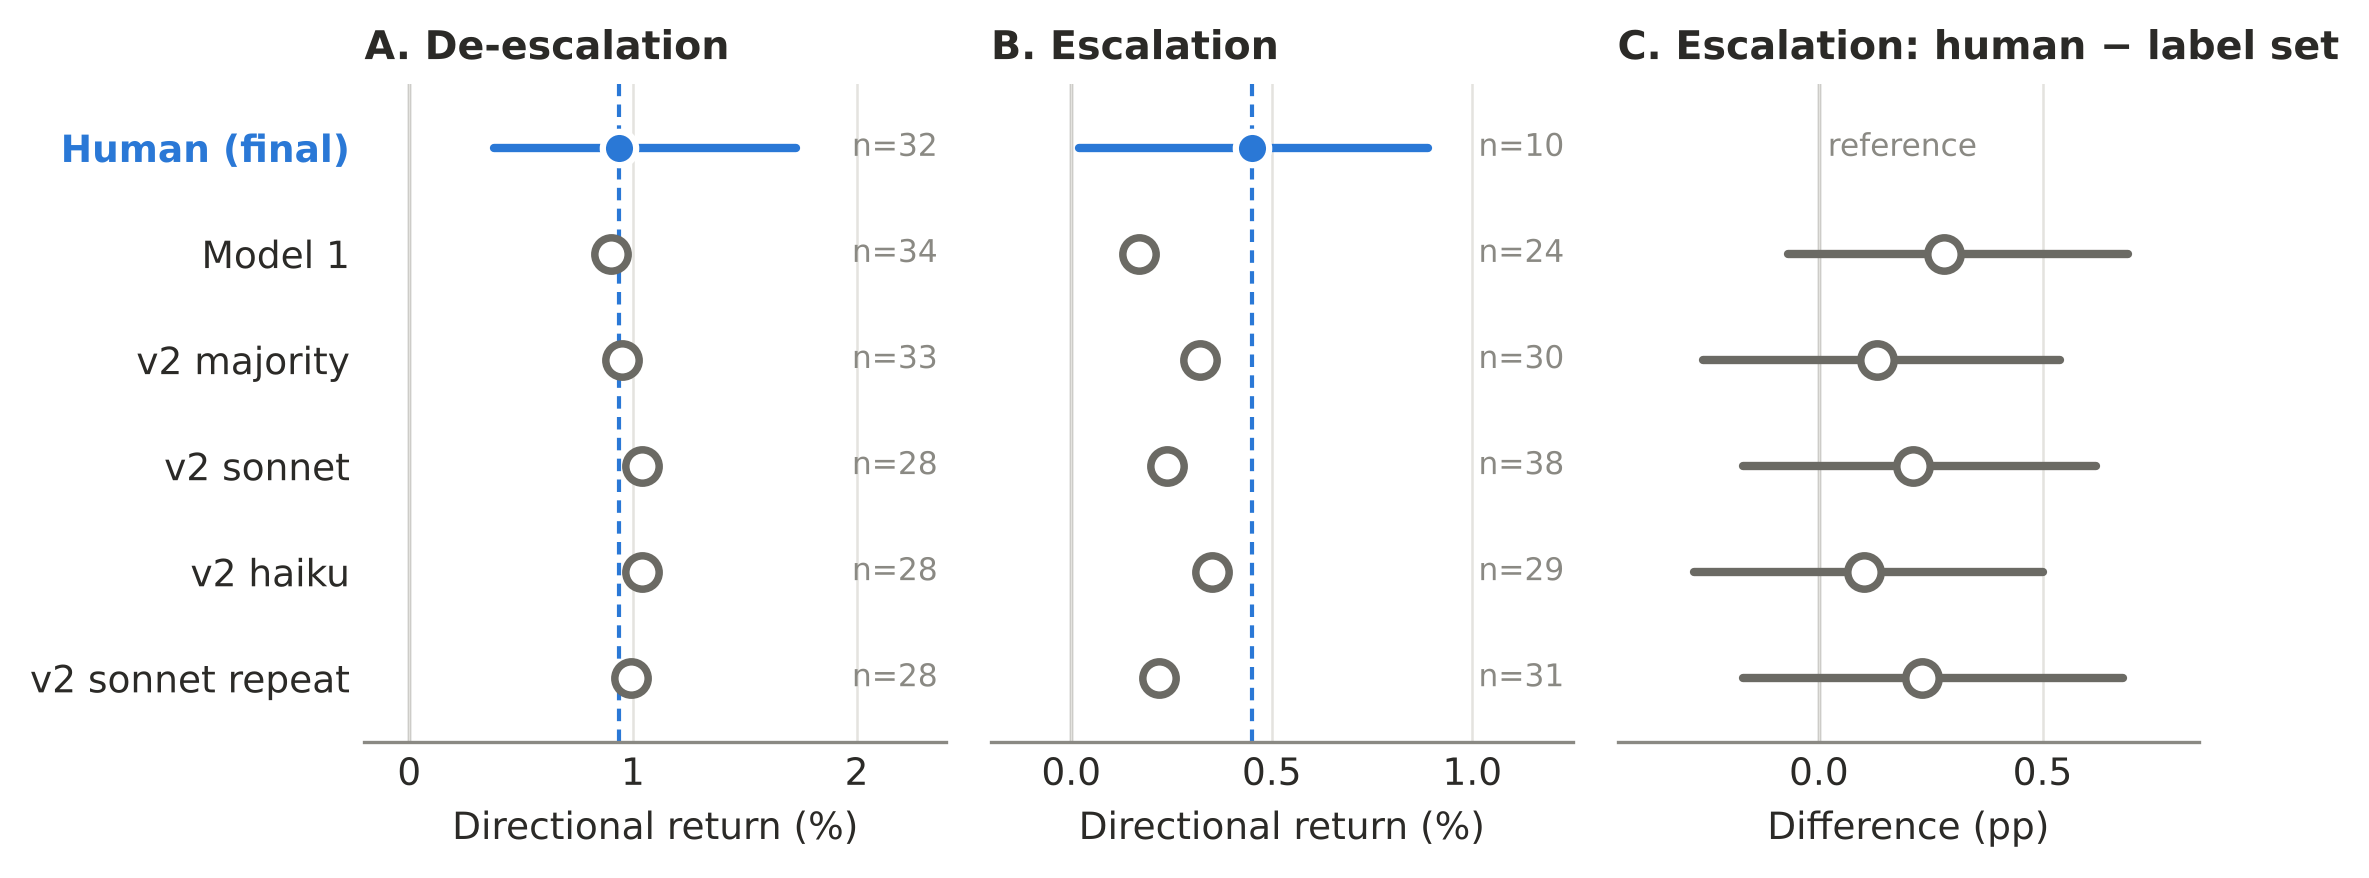
\includegraphics[width=\textwidth]{figures/figure1.png}
\caption{Mean Directional 30-Minute WTI Return by Class Under Each Label Set}
\label{fig:labelsets}
\begin{minipage}{0.95\textwidth}
\footnotesize\textit{Note:} The same 95 events under every label set. Panels A and B: points are mean 30-minute returns signed in the direction of the class; the bar on the human row is its day-clustered bootstrap 95\% confidence interval, and the dashed line marks the human estimate. Numbers at the right give the events in each class. Panel C: human minus label-set escalation estimate, with day-clustered bootstrap 95\% confidence intervals (10,000 resamples). The v2 opus run gives the same results as the v2 majority.
\end{minipage}
\end{figure}

%======================================================================
\section{A Misclassification Decomposition}

Because model and human labels are applied to the same events, the model-label estimate can be written exactly in terms of the human classes. Let $H$ denote the human label of an event, $M$ a model label, and $r_e$ the return signed in the direction of class $e$. The model-label estimate is identically
\begin{equation}
\mu_M(e) \;=\; \sum_{h} \pi(h \mid e)\,\mu(h, e),
\label{eq:mixture}
\end{equation}
where $\pi(h \mid e)$ is the share of the model's class-$e$ events that humans label $h$ (so $\pi(e \mid e)$ is precision), and $\mu(h, e)$ is the mean of $r_e$ over those events. Subtracting the human estimate $\mu_H(e)$ gives
\begin{equation}
\mu_M(e) - \mu_H(e) \;=\; \underbrace{\pi(e \mid e)\,\big[\mu(e, e) - \mu_H(e)\big]}_{\text{selection within the class}} \;+\; \underbrace{\sum_{h \neq e} \pi(h \mid e)\,\big[\mu(h, e) - \mu_H(e)\big]}_{\text{contamination}}.
\label{eq:gap}
\end{equation}
Equation~(\ref{eq:mixture}) is an accounting identity that requires no assumption about the error process, but it makes concrete the result that misclassification bias is a weighted sum of outcome gaps between classes \citep{aigner1973, mahajan2006, lewbel2007}.

Table~\ref{tab:decomp} reports every term for the escalation class. Under model~1, the gap of $-0.28$ points divides into $+0.02$ from selection within the class, $-0.24$ from posts that humans label de-escalation, $+0.02$ from mixed posts, and $-0.08$ from other posts. Under the v2 majority, the gap of $-0.13$ divides into 0.00, $-0.16$, $+0.09$, and $-0.06$.

First, the shortfall is not a weaker response among correctly labelled posts: events that both humans and models call escalation move oil by 0.52\% and 0.44\%, against 0.45\% for the human class.

Second, the largest source of bias is de-escalation posts placed in the escalation class. Six of model~1's 24 escalation events are de-escalation in human judgment; signed as escalation, they move oil by $-0.51$\%, doing more damage than an unrelated post, which contributes roughly zero.

Third, precision does not predict bias. The v2 majority is slightly less precise than model~1 on these events (9 of 30, against 8 of 24), yet its bias is less than half as large, because its errors come from different places. Most of its added posts are mixed posts, in which humans also see a threat and which move oil in the escalation direction ($+0.68$\%), and fewer are de-escalation posts (4 against 6). Label sets with similar $\kappa$ and precision can thus bias an estimate by different amounts.

The identity also explains why the de-escalation estimate is stable: precision is higher and no human escalation post enters the class (SI Table S3). Because its terms can be estimated on any validated subsample, it doubles as a diagnostic. It is relative to human labels that are themselves measured with error, so it does not recover the true response; a latent-class extension with several raters per post is identified under conditions on how raters' errors relate \citep{hu2008}. We wrote the decomposition after the event-level split was known (post hoc; SI Section S7).

\begin{table}[t]
\centering
\small
\caption{Misclassification Decomposition of the Escalation Estimate}
\label{tab:decomp}
\begin{tabular}{lcc}
\toprule
 & Model 1 & v2 majority \\
\midrule
Model-labelled escalation events & 24 & 30 \\
\quad Human escalation (same class) & 8 ($+0.52$) & 9 ($+0.44$) \\
\quad Human de-escalation & 6 ($-0.51$) & 4 ($-0.75$) \\
\quad Human mixed & 7 ($+0.52$) & 12 ($+0.68$) \\
\quad Human other & 3 ($-0.21$) & 5 ($+0.09$) \\
\midrule
Mean, eq.~(\ref{eq:mixture}) & $+0.17$ & $+0.32$ \\
Human estimate $\mu_H(e)$ & $+0.45$ & $+0.45$ \\
\textbf{Gap, eq.~(\ref{eq:gap})} & $\mathbf{-0.28}$ & $\mathbf{-0.13}$ \\
\quad Selection within the class & $+0.02$ & $0.00$ \\
\quad Contamination: de-escalation & $-0.24$ & $-0.16$ \\
\quad Contamination: mixed & $+0.02$ & $+0.09$ \\
\quad Contamination: other & $-0.08$ & $-0.06$ \\
\bottomrule
\end{tabular}

\vspace{0.5em}
\begin{minipage}{0.85\textwidth}
\footnotesize\textit{Note:} Same 95-event frame. Final human labels (10 escalation events). Cells give the number of model-labelled escalation events with each human label and, in parentheses, their mean 30-minute WTI return (percent), signed in the escalation direction. Components are rounded and need not sum exactly. The corresponding decomposition for the de-escalation class is in SI Table S3.
\end{minipage}
\end{table}

%======================================================================
\section{How Much Validation Is Enough?}

Prediction-powered inference \citep{angelopoulos2023} and design-based supervised learning \citep[DSL;][]{egami2023} correct model-label estimates with human labels for a random subsample. In an exploratory simulation that validated 10\% to 50\% of posts (SI Section S5), DSL removed the bias but, with ten escalation events, became more accurate than the naive model-label estimate only once about 30\% of posts were validated with model~1 labels, and not even at 50\% with the better v2 majority labels. A validated subsample is not a cheap fix when events are few.

%======================================================================
\section{Recommendations and Limits}

We suggest four reporting practices.

\begin{enumerate}
\item \textbf{Report validity by class, not only consistency.} Report agreement between runs as reliability, and agreement with human coders for each class, with a prevalence-robust measure alongside $\kappa$ and with precision and recall for the classes analysed.
\item \textbf{Give models and humans the same instructions.} State who wrote the codebook, when, and with what knowledge of earlier errors.
\item \textbf{Compare and decompose.} Estimate the downstream quantity under alternative label sets on the same units, and decompose any difference with equation~(\ref{eq:gap}).
\item \textbf{Check whether correction pays at the available scale}, by simulation on the validated subsample.
\end{enumerate}

Our evidence has clear limits. It comes from one episode, one sender, and one asset, and the escalation result rests on ten events. Half of the escalation signal posts were made while the market was closed and are lost, against 18\% of de-escalation posts. The human labels are a moderately reliable benchmark formed with hindsight. We tested one model family under default settings. The decomposition and simulation were designed after the main results were known, and the event sample was redefined as label quality became clear; the SI documents each version.

An analysis that reported only the agreement between model runs would have certified labels that changed the answer. Agreement with human readers, not agreement between model runs, is the evidence a labelling needs before it enters downstream inference.

\clearpage
\section*{Data Availability Statement}
\chk{Replication code, prompts, model outputs, coder sheets, and analysis plans will be deposited in the Political Analysis Dataverse. Post texts come from a public archive; tick data are from Dukascopy (check redistribution terms).}

\section*{Use of Generative AI}
Large language models were used as classification instruments, as described in Section~2 and the SI. \chk{State any use of generative AI in writing or coding, consistent with the journal's policy.}

\bibliographystyle{apalike}
\bibliography{references}

\end{document}
